% Example 

%%%%%%%%%
% Purpose

\def\keradius{
\begin{figure}[h]
    \centering
    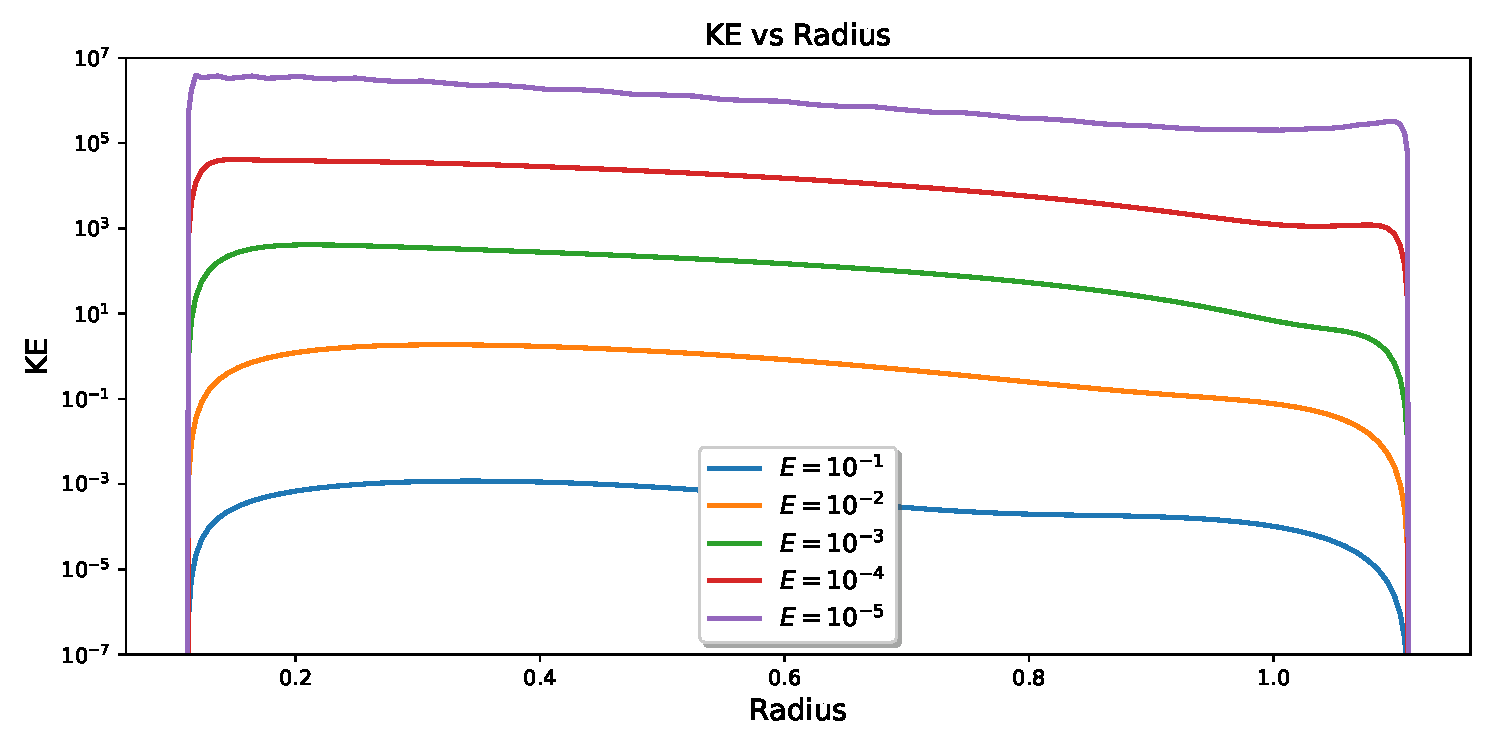
\includegraphics[width=1\textwidth]{figures/ke_radius_all.pdf}
    \caption{Kinetic energy shell average as a function of radius during equilibrated phase for a range of Ekman numbers.}
    \label{fig:ke_radius}
\end{figure}
}


\def\azavgtemperature{
\begin{figure}[h]
    \centering
    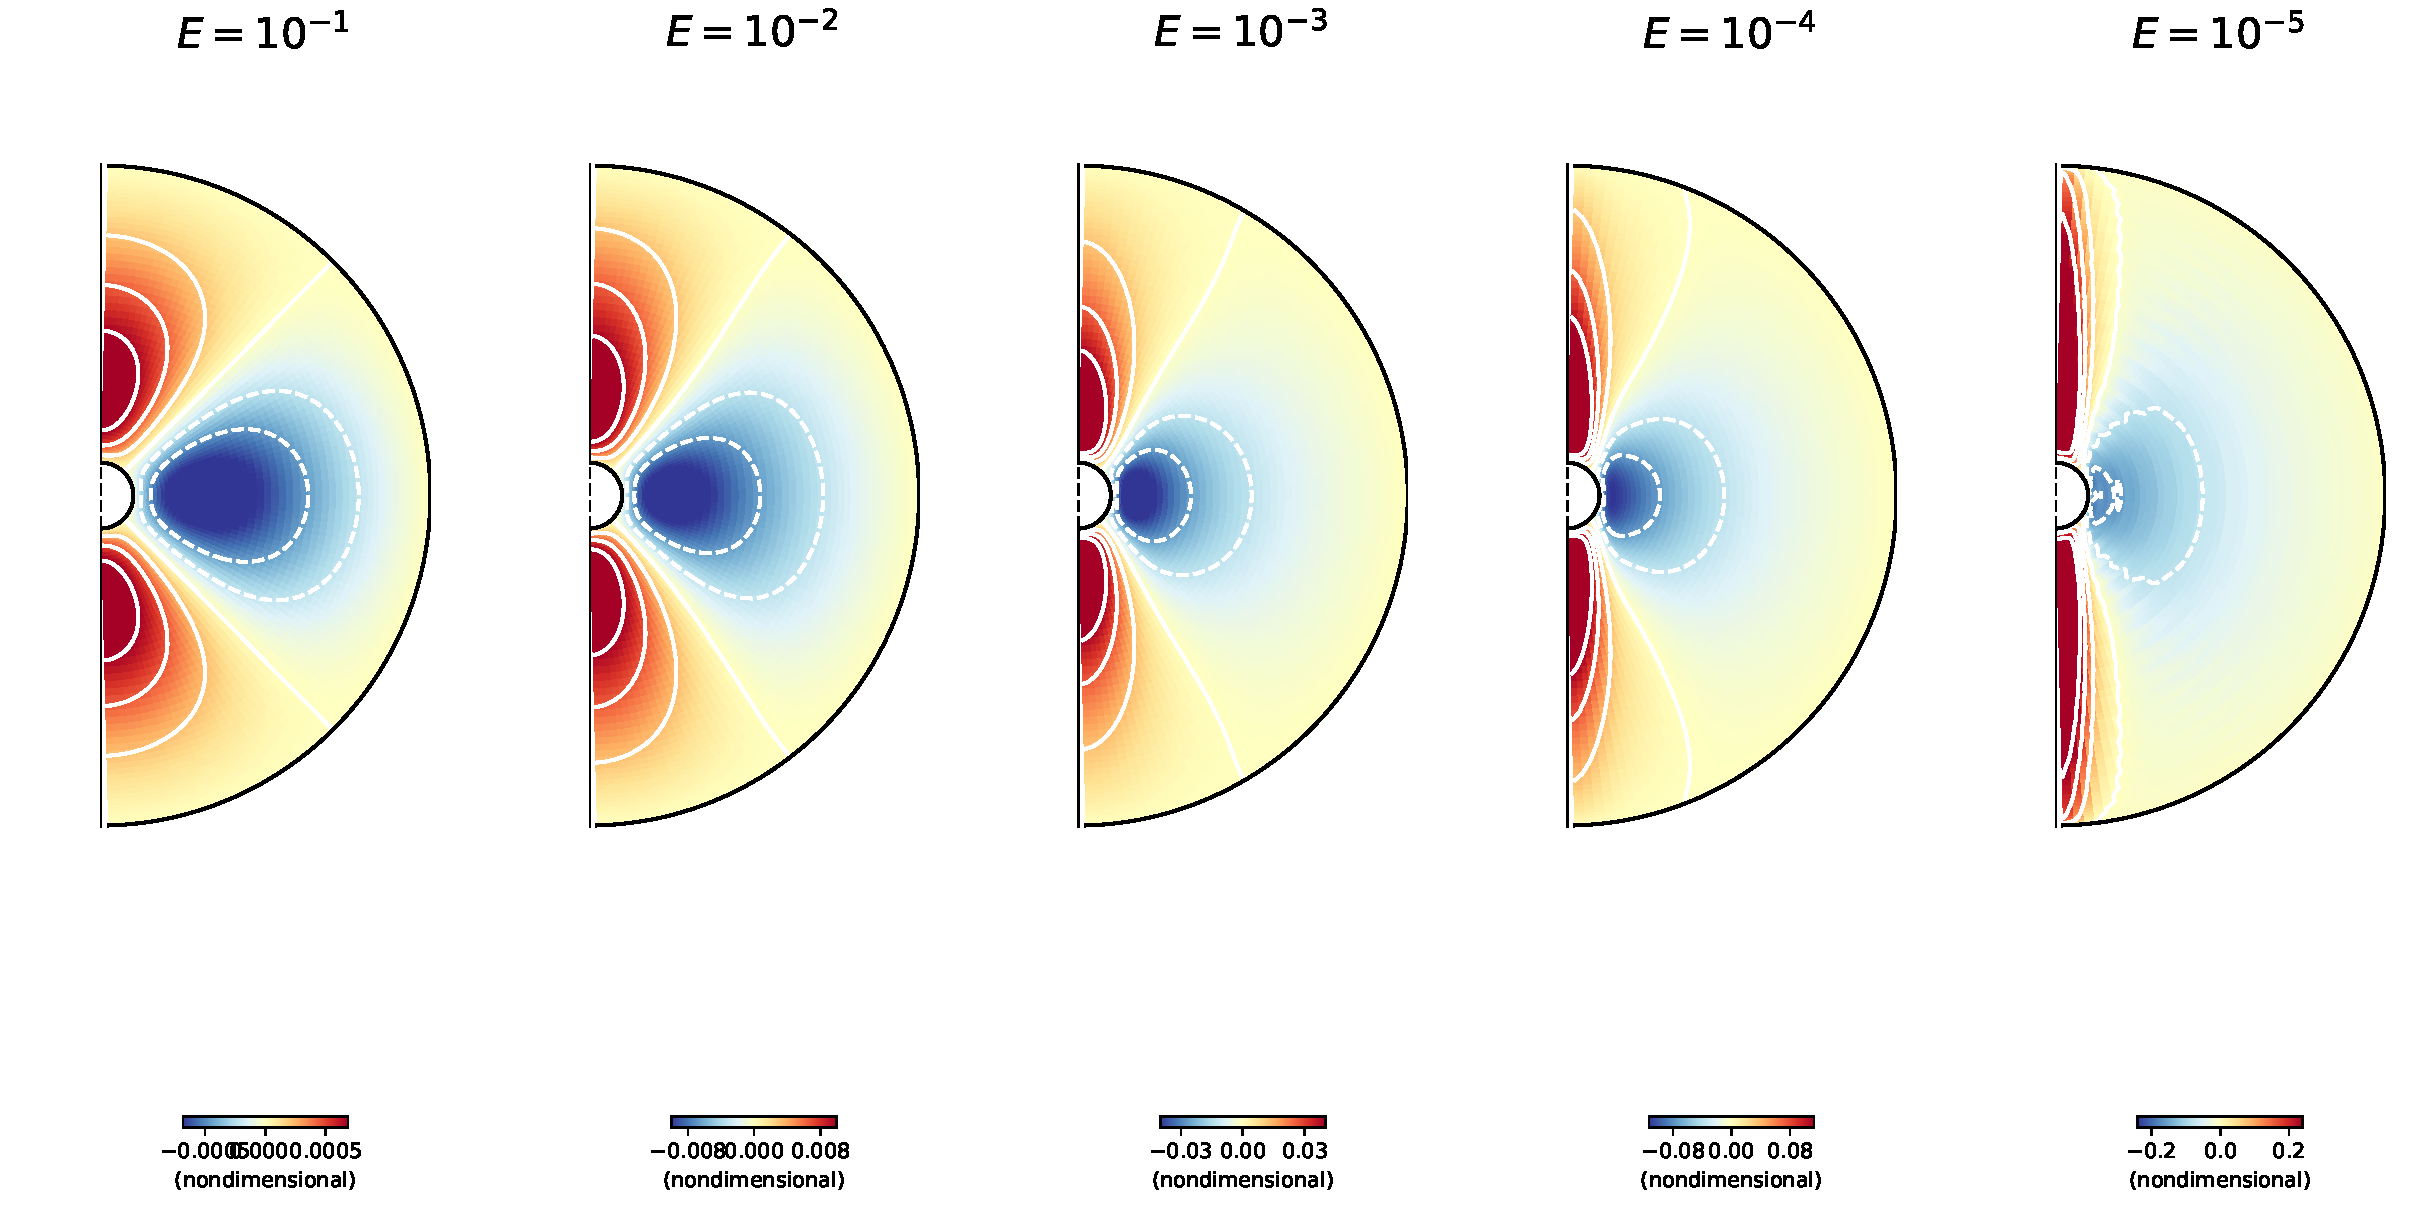
\includegraphics[width=1\textwidth]{figures/AZ_Avgs_501.pdf}
    \caption{Temperature azimuthal average during equilibrated phase for a range of Ekman numbers.}
    \label{fig:az_avg_temperature}
\end{figure}
}

\def\azavgomega{
\begin{figure}[h]
    \centering
    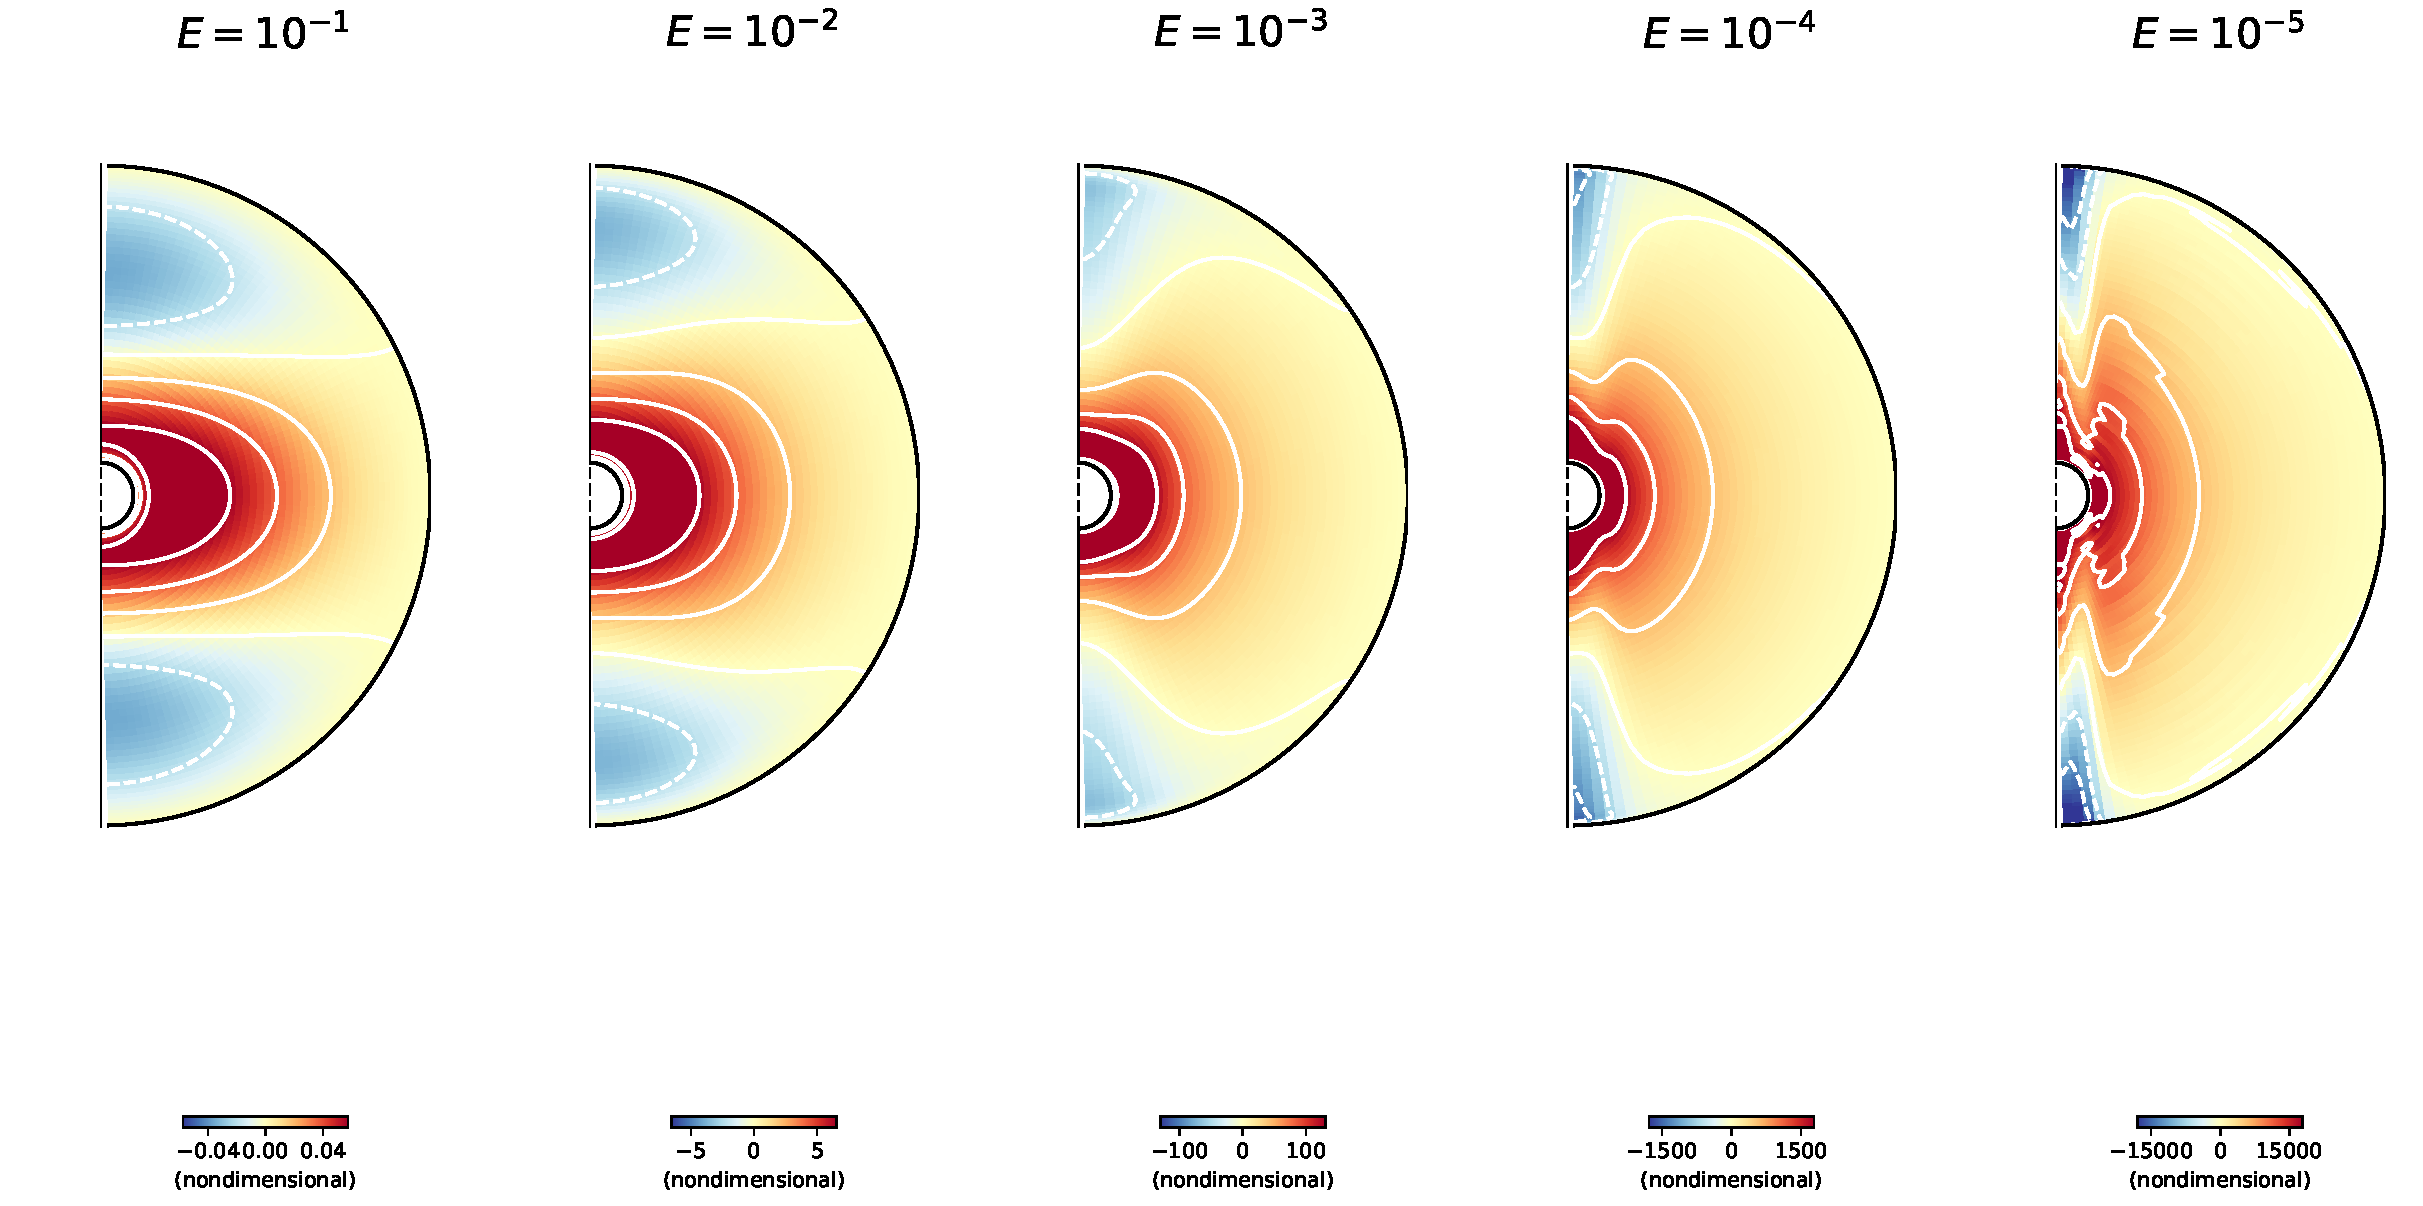
\includegraphics[width=1\textwidth]{figures/AZ_Avgs_omega.pdf}
    \caption{Angular velocity azimuthal average during equilibrated phase for a range of Ekman numbers.}
    \label{fig:az_avg_omega}
\end{figure}
}

\def\azavgmassflux{
\begin{figure}[h]
    \centering
    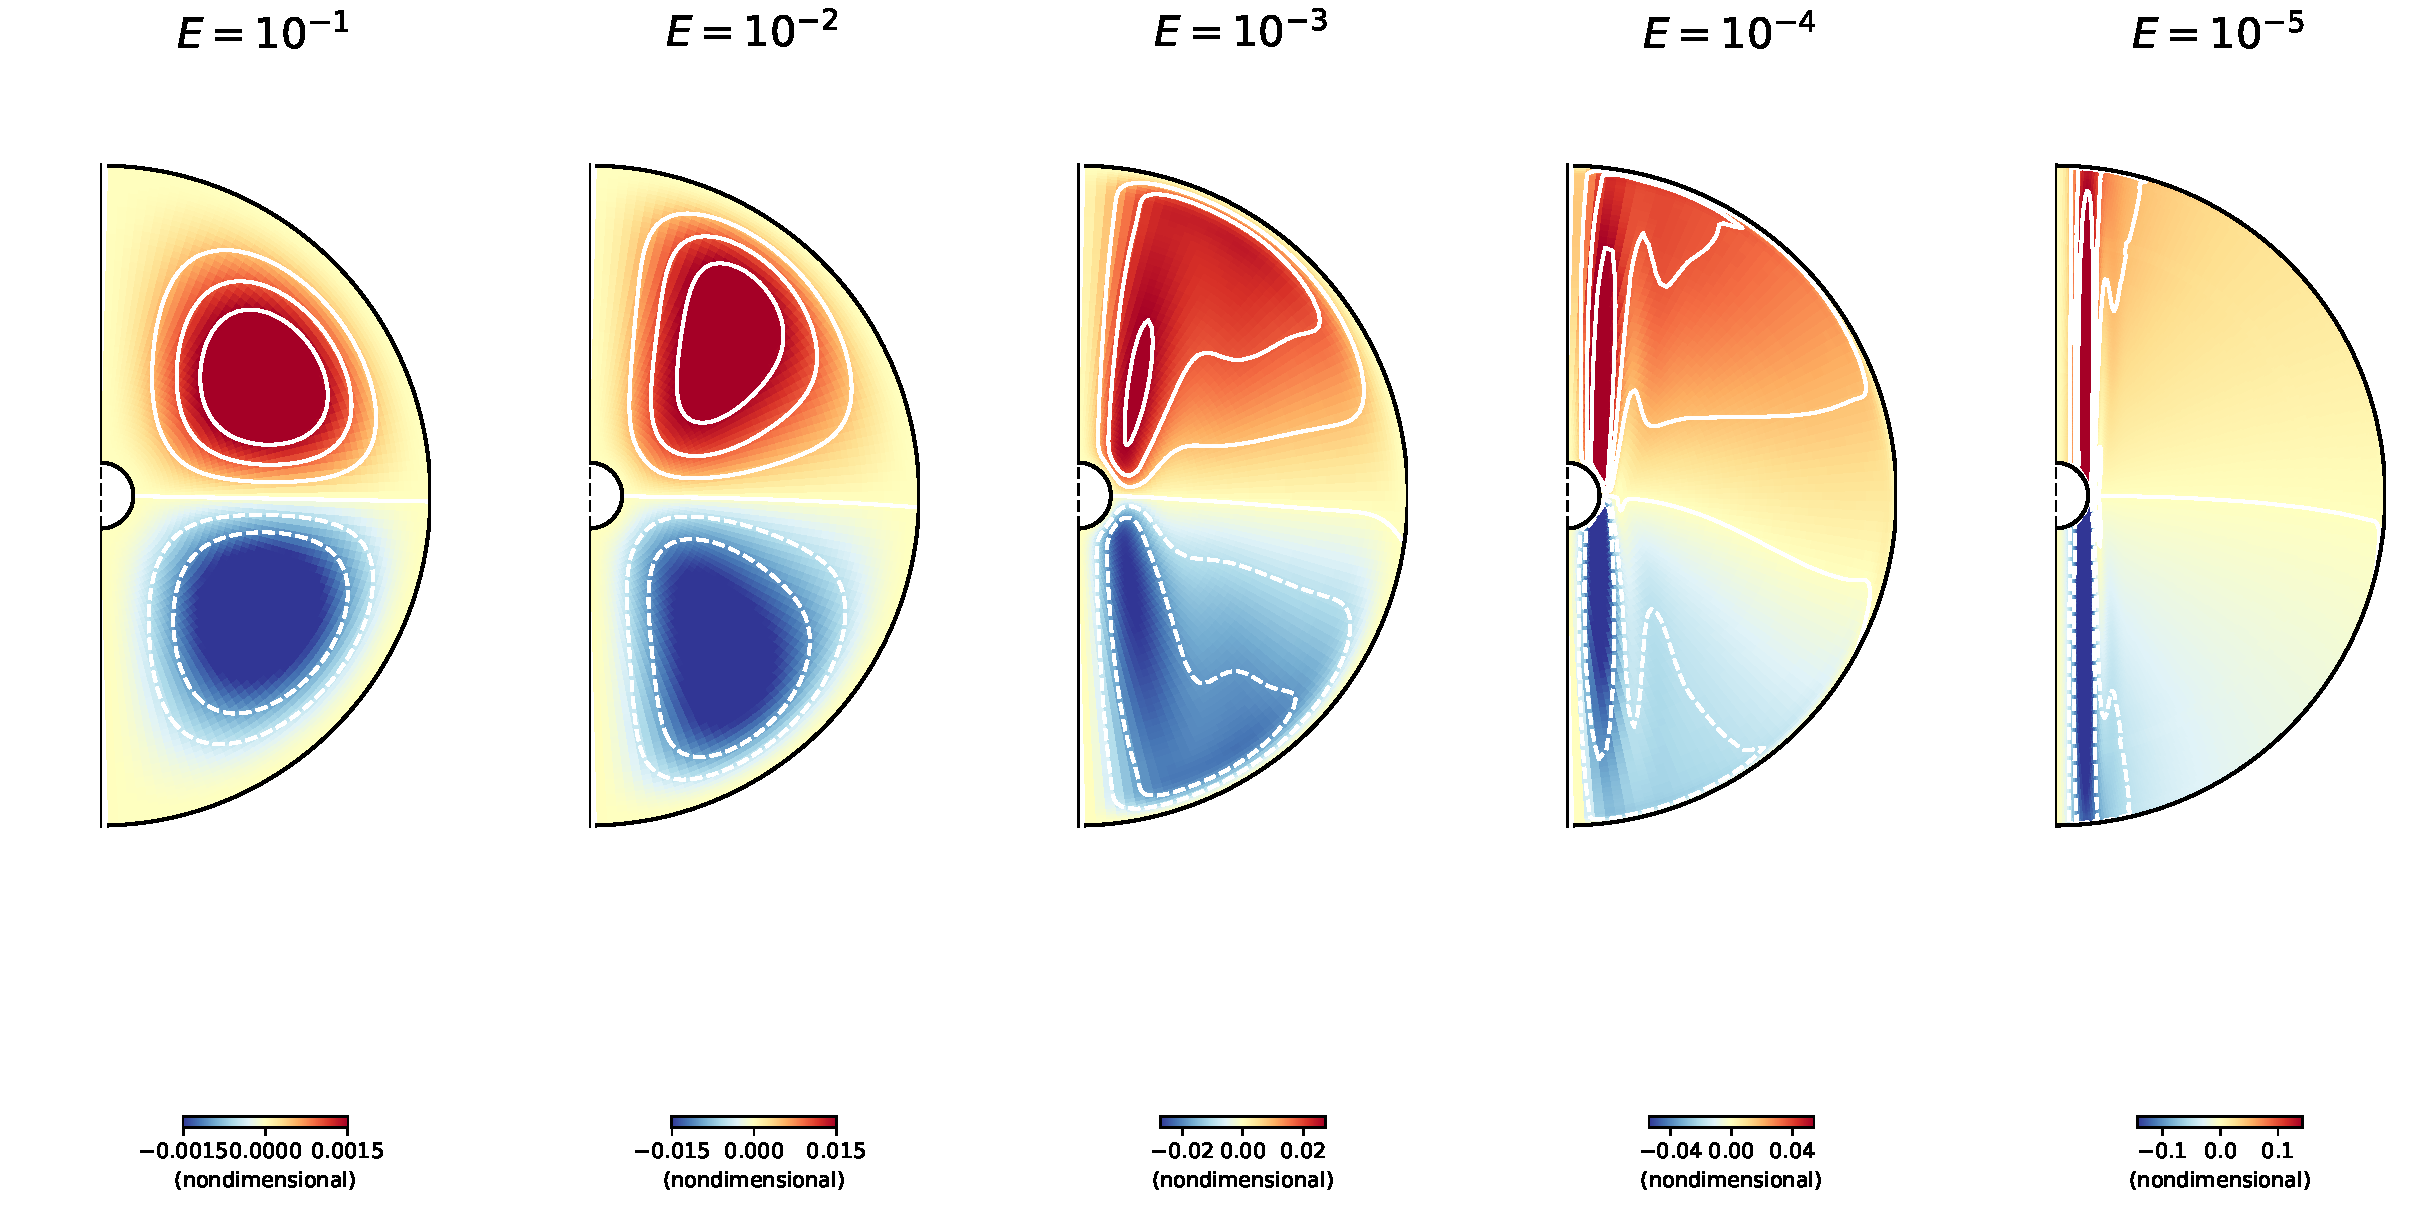
\includegraphics[width=1\textwidth]{figures/AZ_Avgs_psi.pdf}
    \caption{Mass flux azimuthal average during equilibrated phase for a range of Ekman numbers.}
    \label{fig:az_avg_massflux}
\end{figure}
}

\def\fluxpol{
\begin{figure}[h]
    \centering
    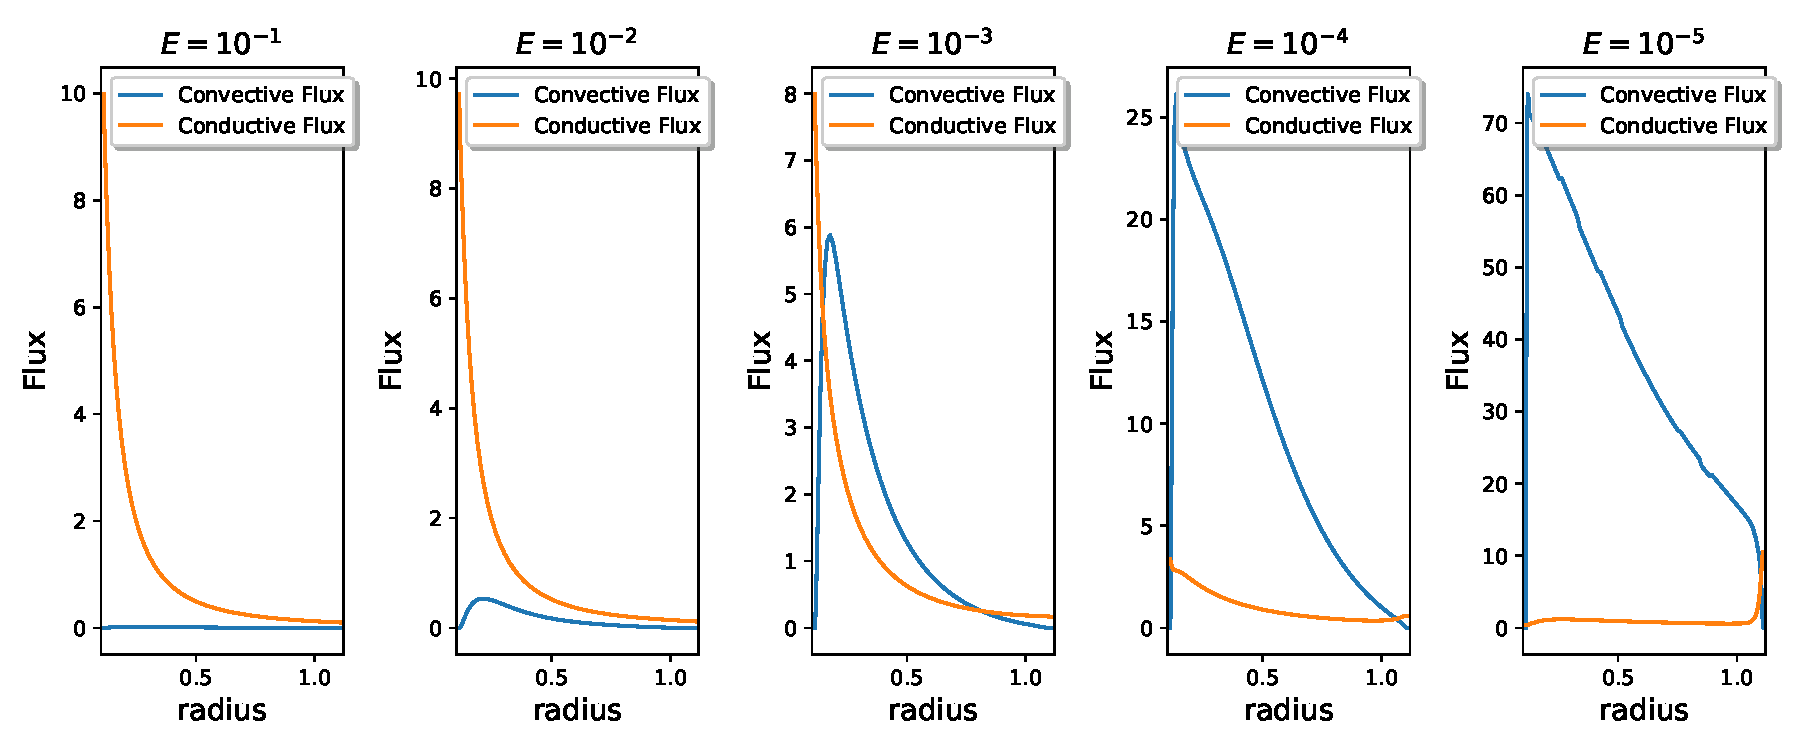
\includegraphics[width=1\textwidth]{figures/flux_radius_all_pol.pdf}
    \caption{Azimuthal average of convective and conductive heat flux at the pole for a range of Ekman numbers.}
    \label{fig:flux_pol}
\end{figure}
}

\def\fluxeq{
\begin{figure}[h]
    \centering
    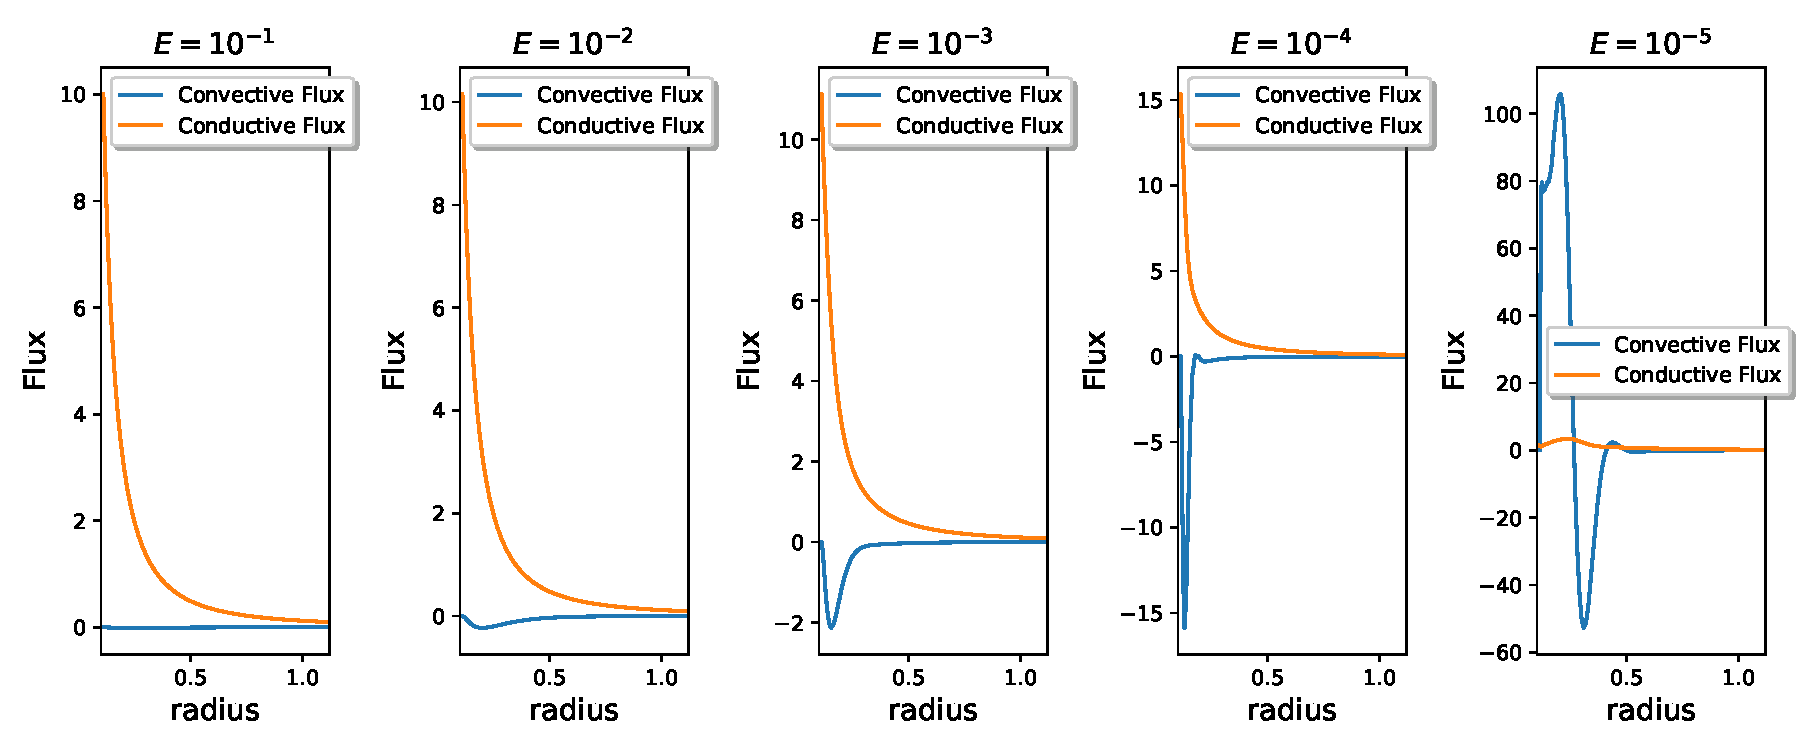
\includegraphics[width=1\textwidth]{figures/flux_radius_all_eq.pdf}
    \caption{Azimuthal average of convective and conductive heat flux at the equator for a range of Ekman numbers.}
    \label{fig:flux_eq}
\end{figure}
}

\def\condfluxrin{
\begin{figure}[h]
    \centering
    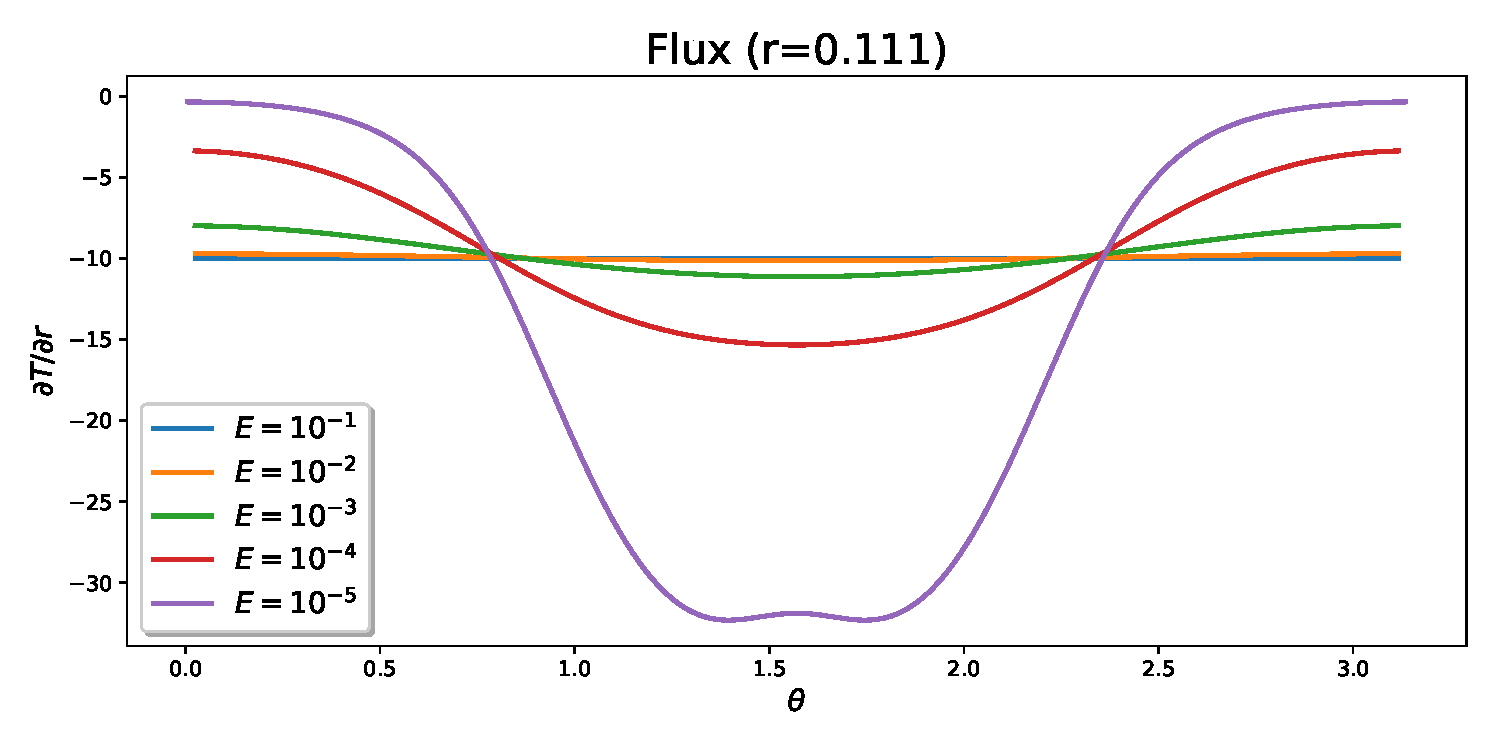
\includegraphics[width=1\textwidth]{figures/condflux_theta_rin.pdf}
    \caption{Conductive flux azimuthal average as a function of $\theta$ at the inner radius for a range of Ekman numbers.}
    \label{fig:condflux_rin}
\end{figure}
}


\def\condfluxrout{
\begin{figure}[h]
    \centering
    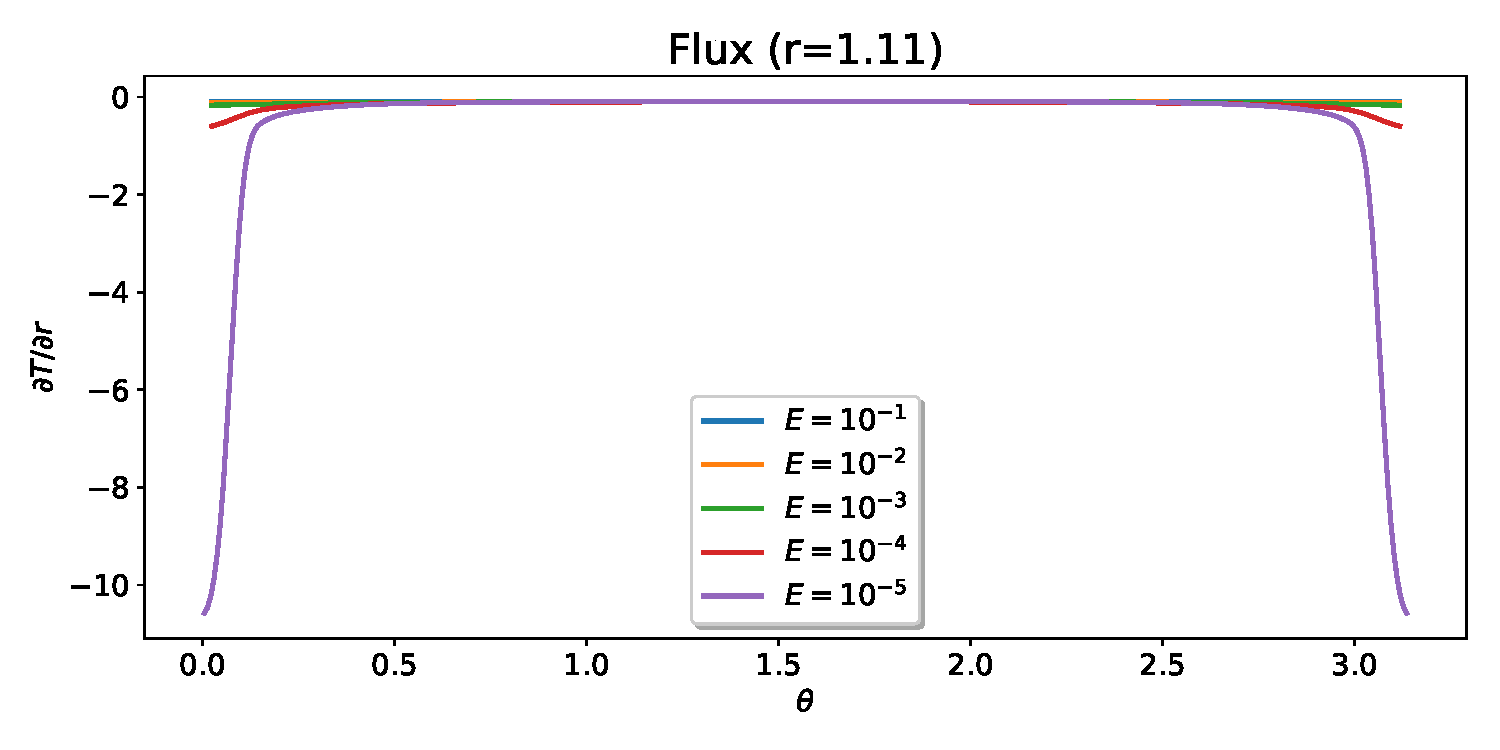
\includegraphics[width=1\textwidth]{figures/condflux_theta_rout.pdf}
    \caption{Conductive flux azimuthal average as a function of $\theta$ at the outer radius for a range of Ekman numbers.}
    \label{fig:condflux_rout}
\end{figure}
}


%%%%%%%%%%%%%%%
% AR_0.5 section

\def\keradiusarfive{
\begin{figure}[h]
    \centering
	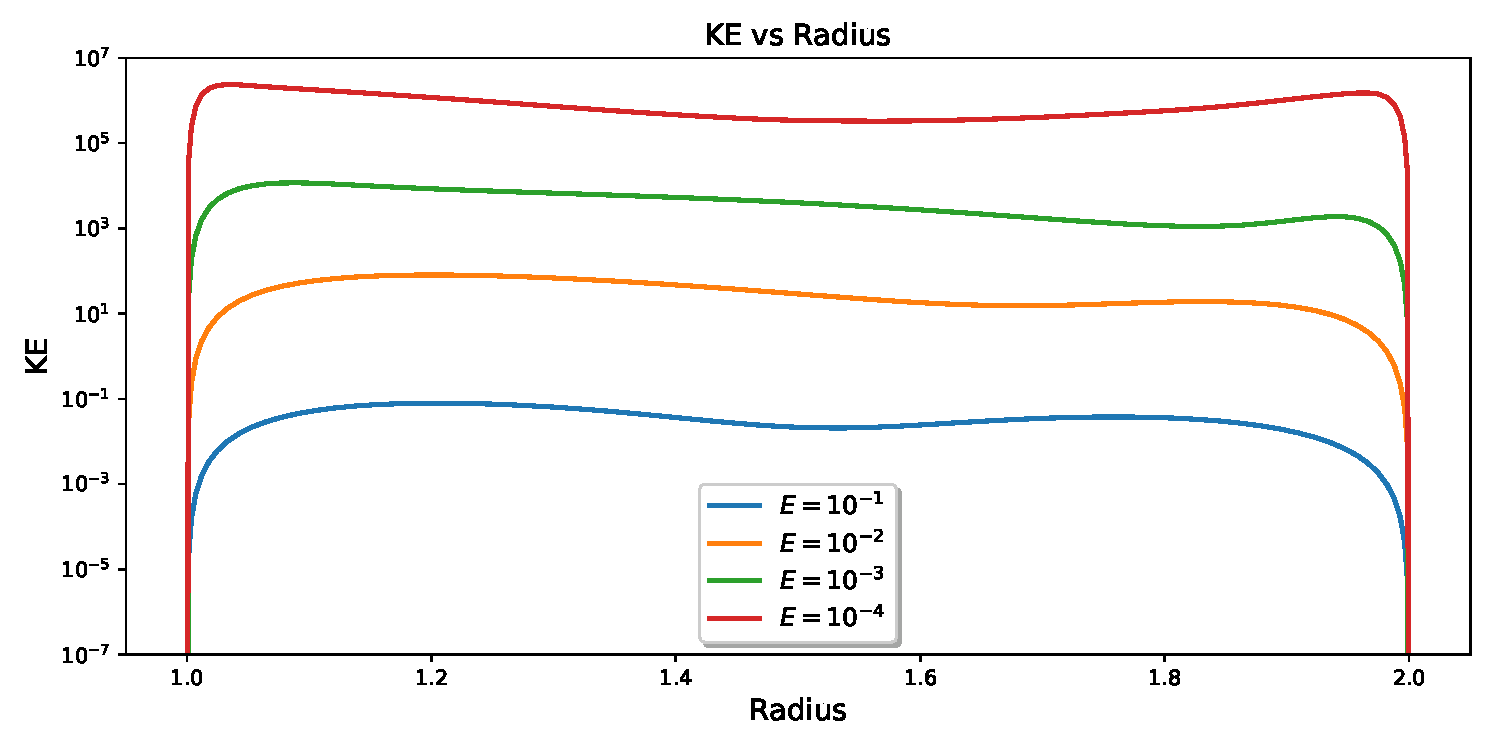
\includegraphics[width=1\textwidth]{figures/AR_0.5/ke_radius_all_ar0p5.pdf}
    \caption{Kinetic energy shell average as a function of radius during equilibrated phase for a range of Ekman numbers with aspect ratio set to 0.5.}
    \label{fig:ke_radius_ar_0.5}
\end{figure}
}

\def\azavgtemperaturearfive{
\begin{figure}[h]
    \centering
    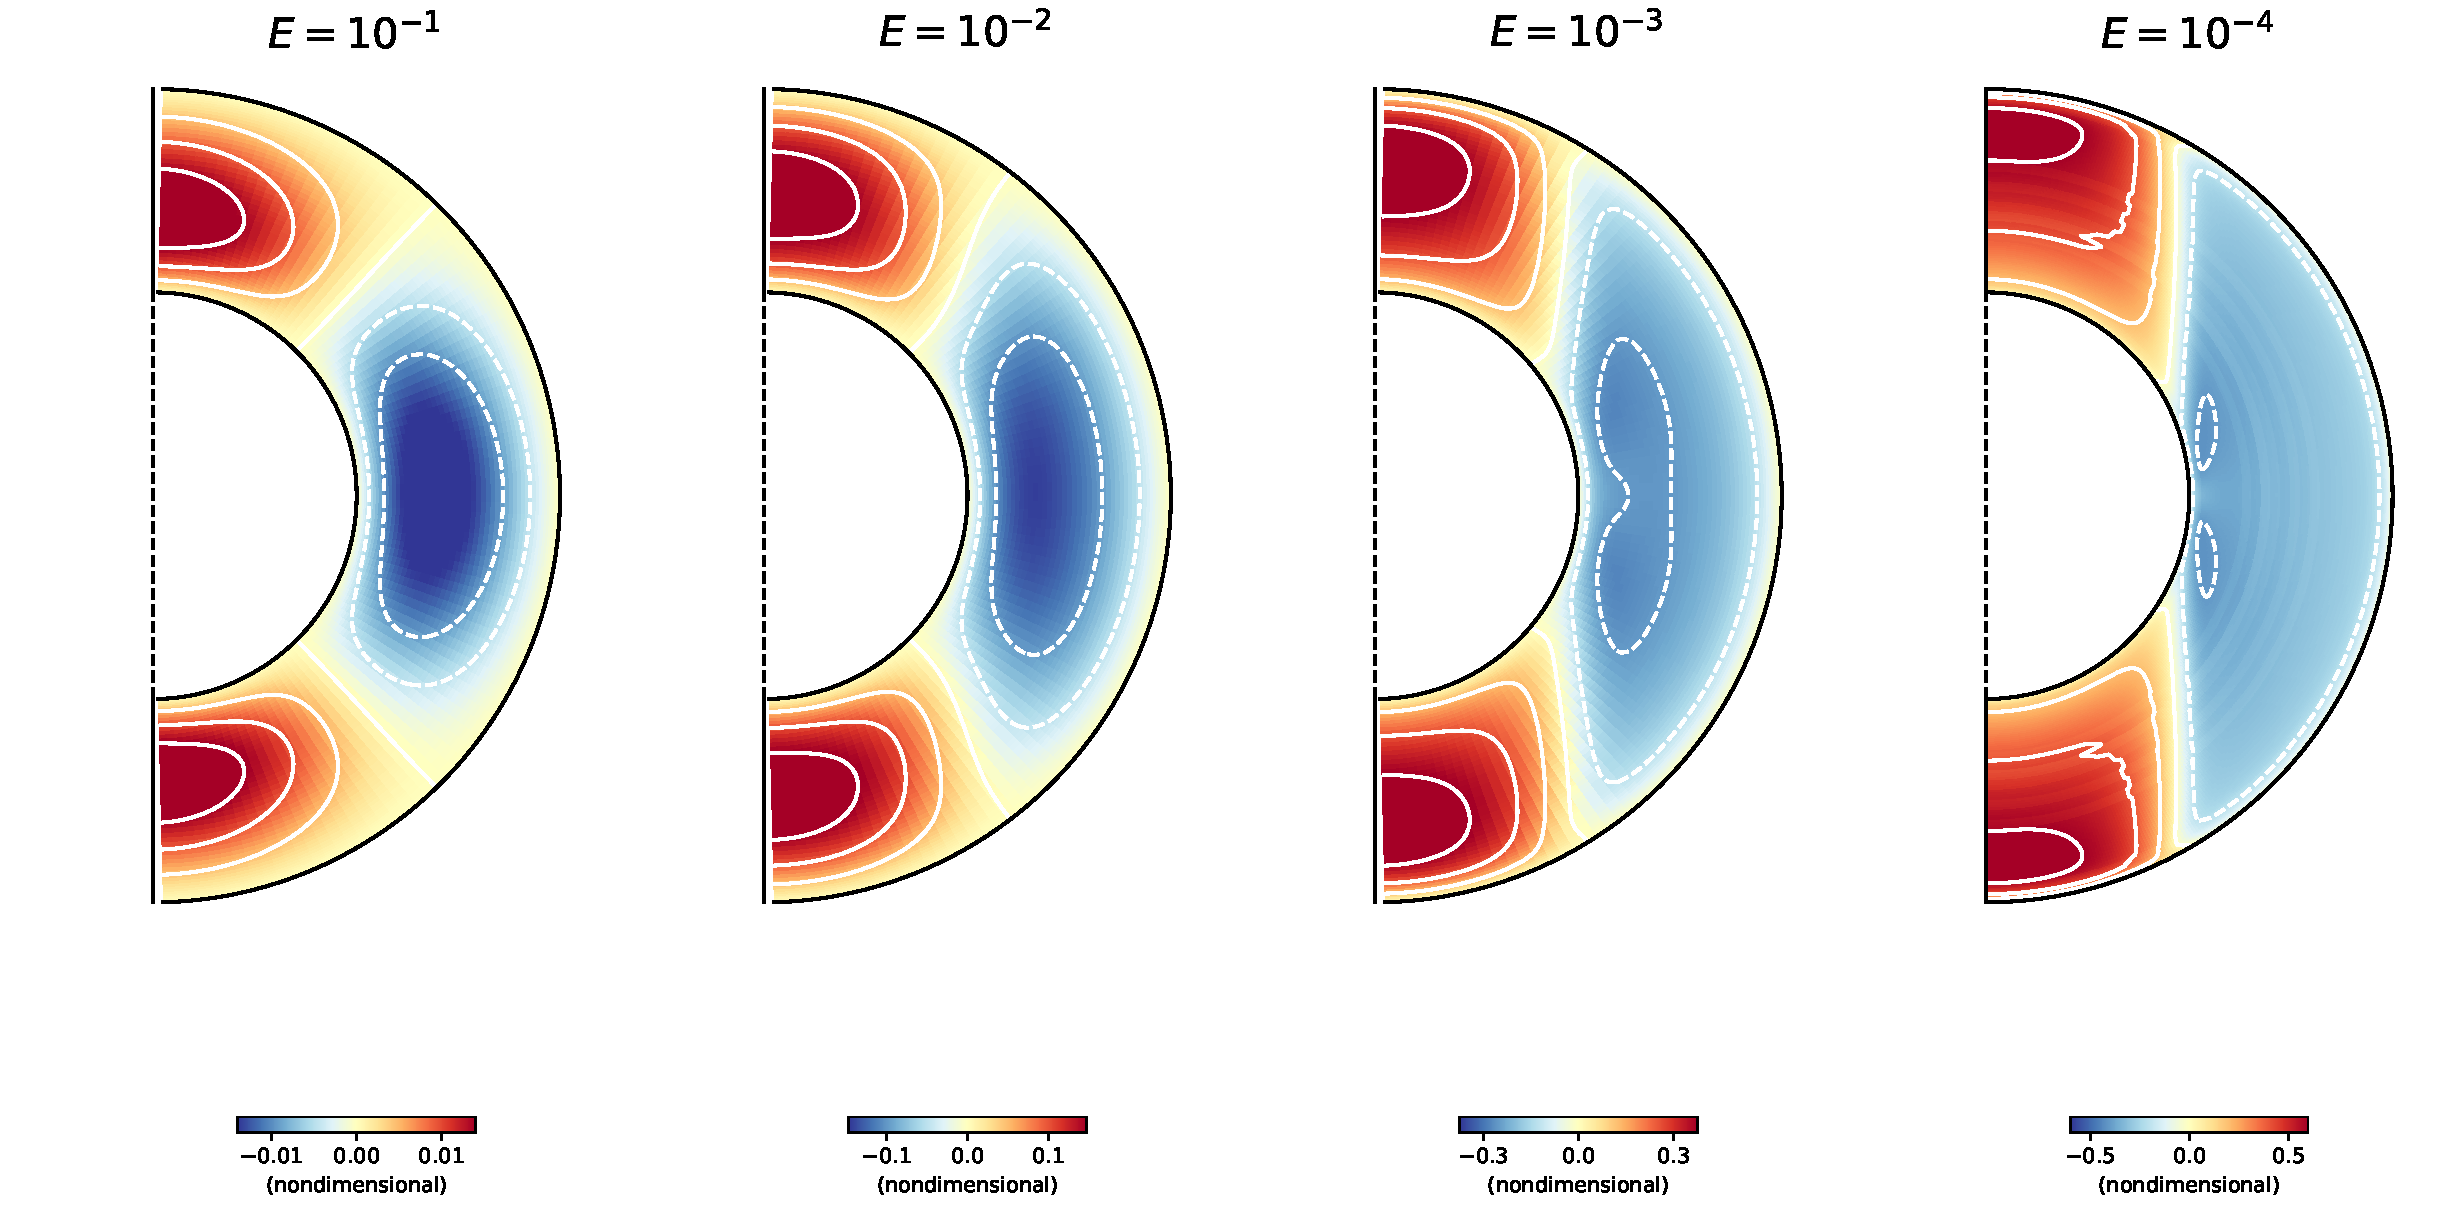
\includegraphics[width=1\textwidth]{figures/AR_0.5/AZ_Avgs_temperature_ar0p5.pdf}
    \caption{Temperature azimuthal average during equilibrated phase for a range of Ekman numbers.}
    \label{fig:az_avg_temperature_ar0.5}
\end{figure}
}

\def\azavgomegaarfive{
\begin{figure}[h]
    \centering
    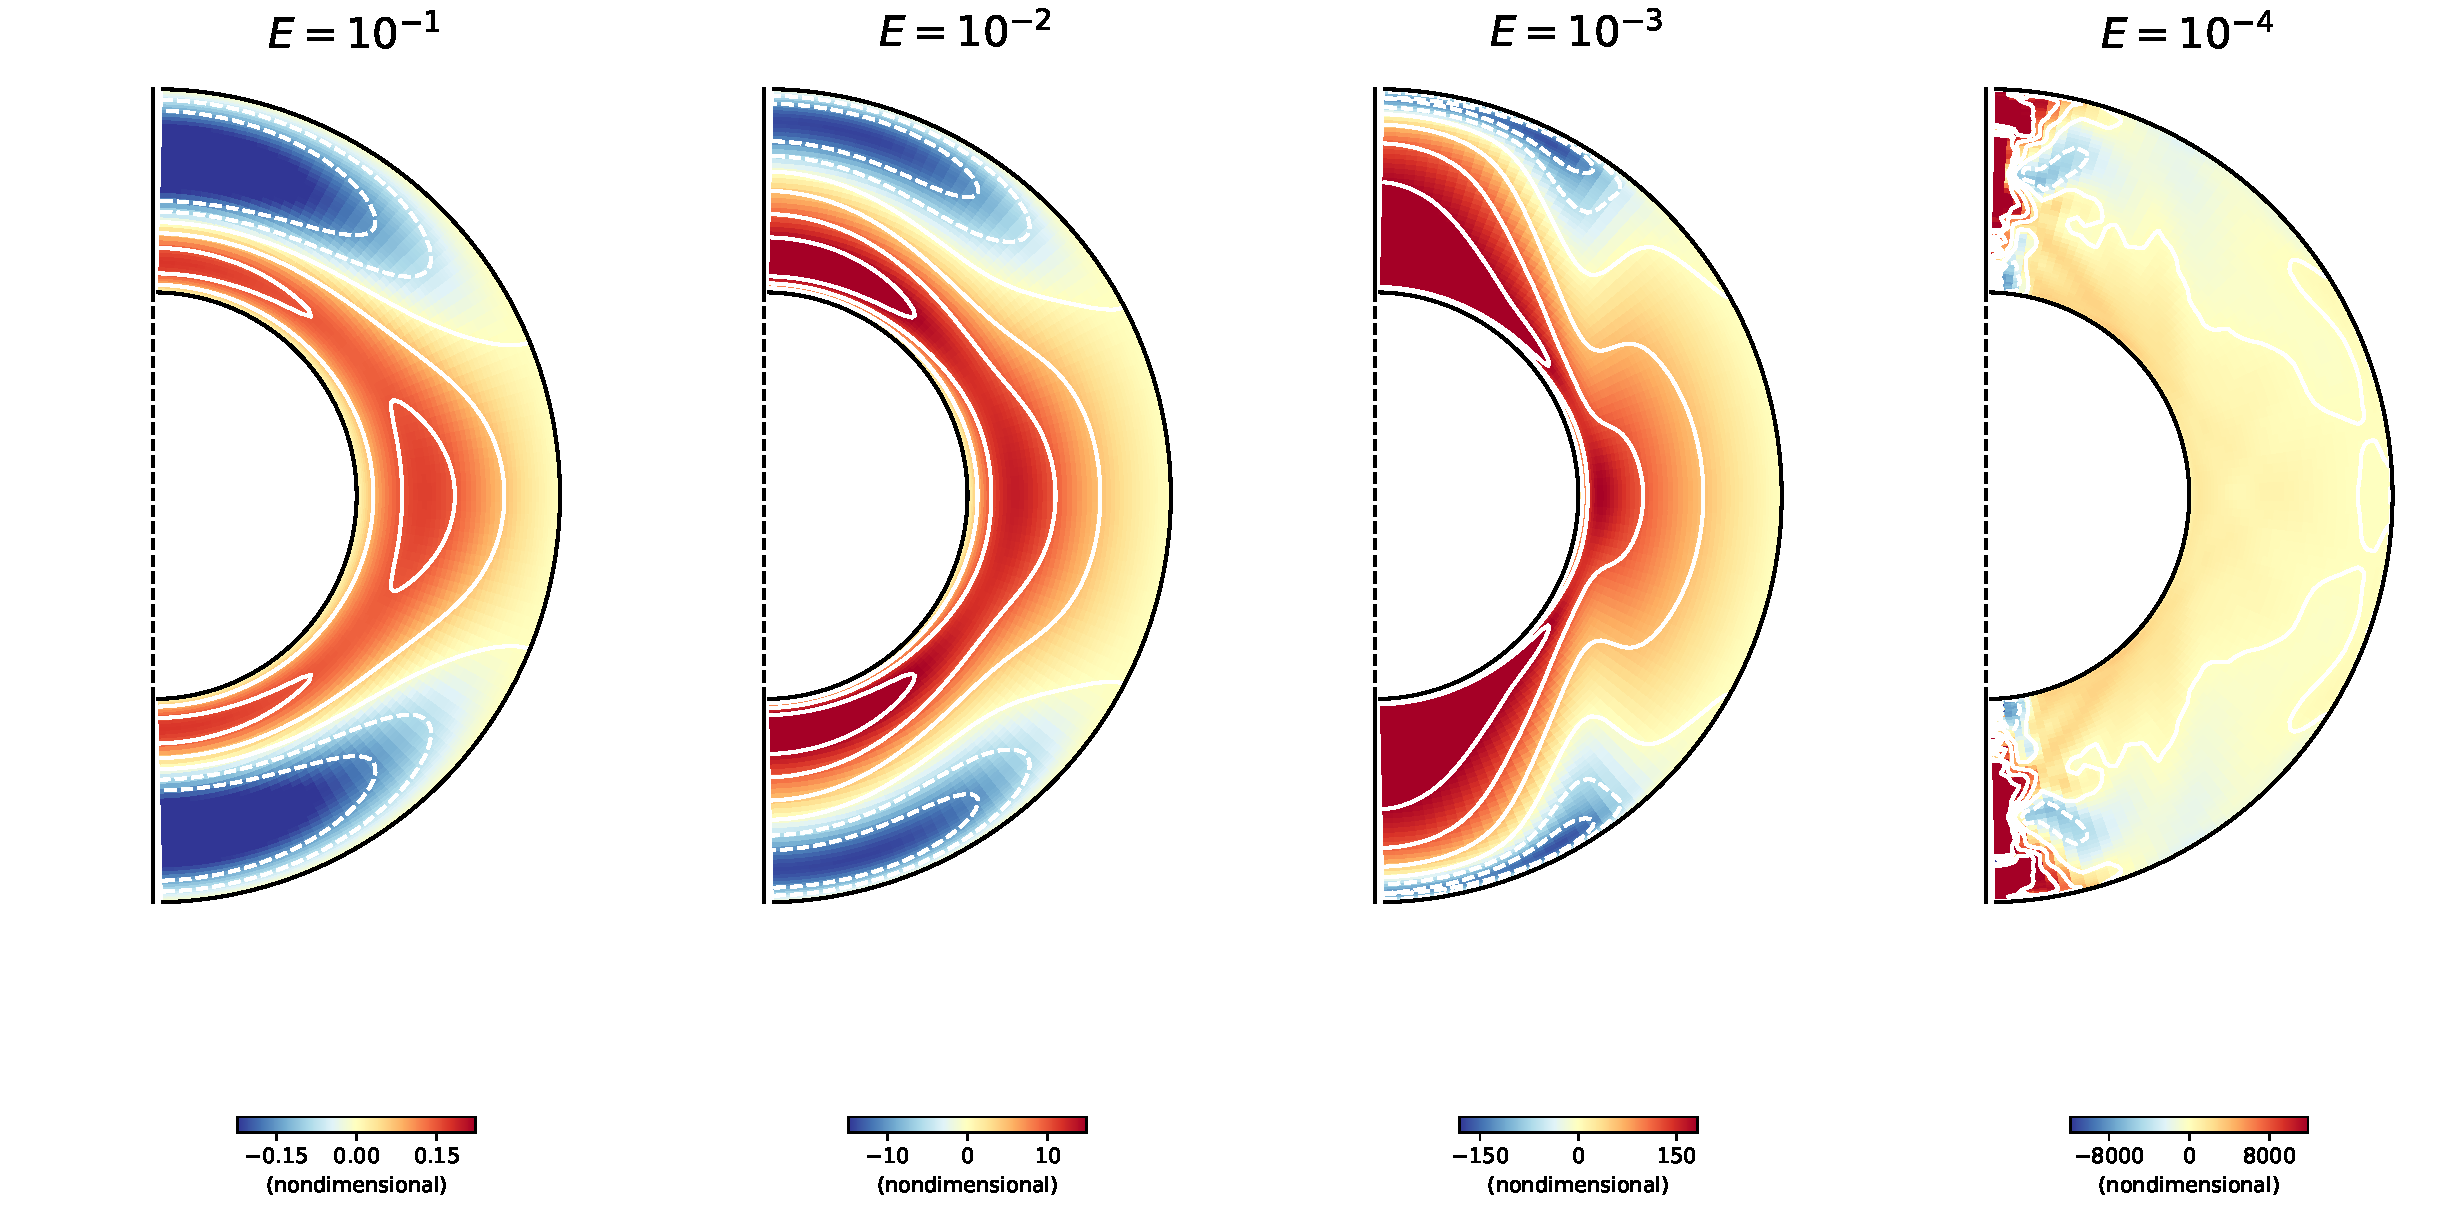
\includegraphics[width=1\textwidth]{figures/AR_0.5/AZ_Avgs_omega_ar0p5.pdf}
    \caption{Angular velocity azimuthal average during equilibrated phase for a range of Ekman numbers.}
    \label{fig:az_avg_omega_ar_0.5}
\end{figure}
}

\def\azavgmassfluxarfive{
\begin{figure}[h]
    \centering
    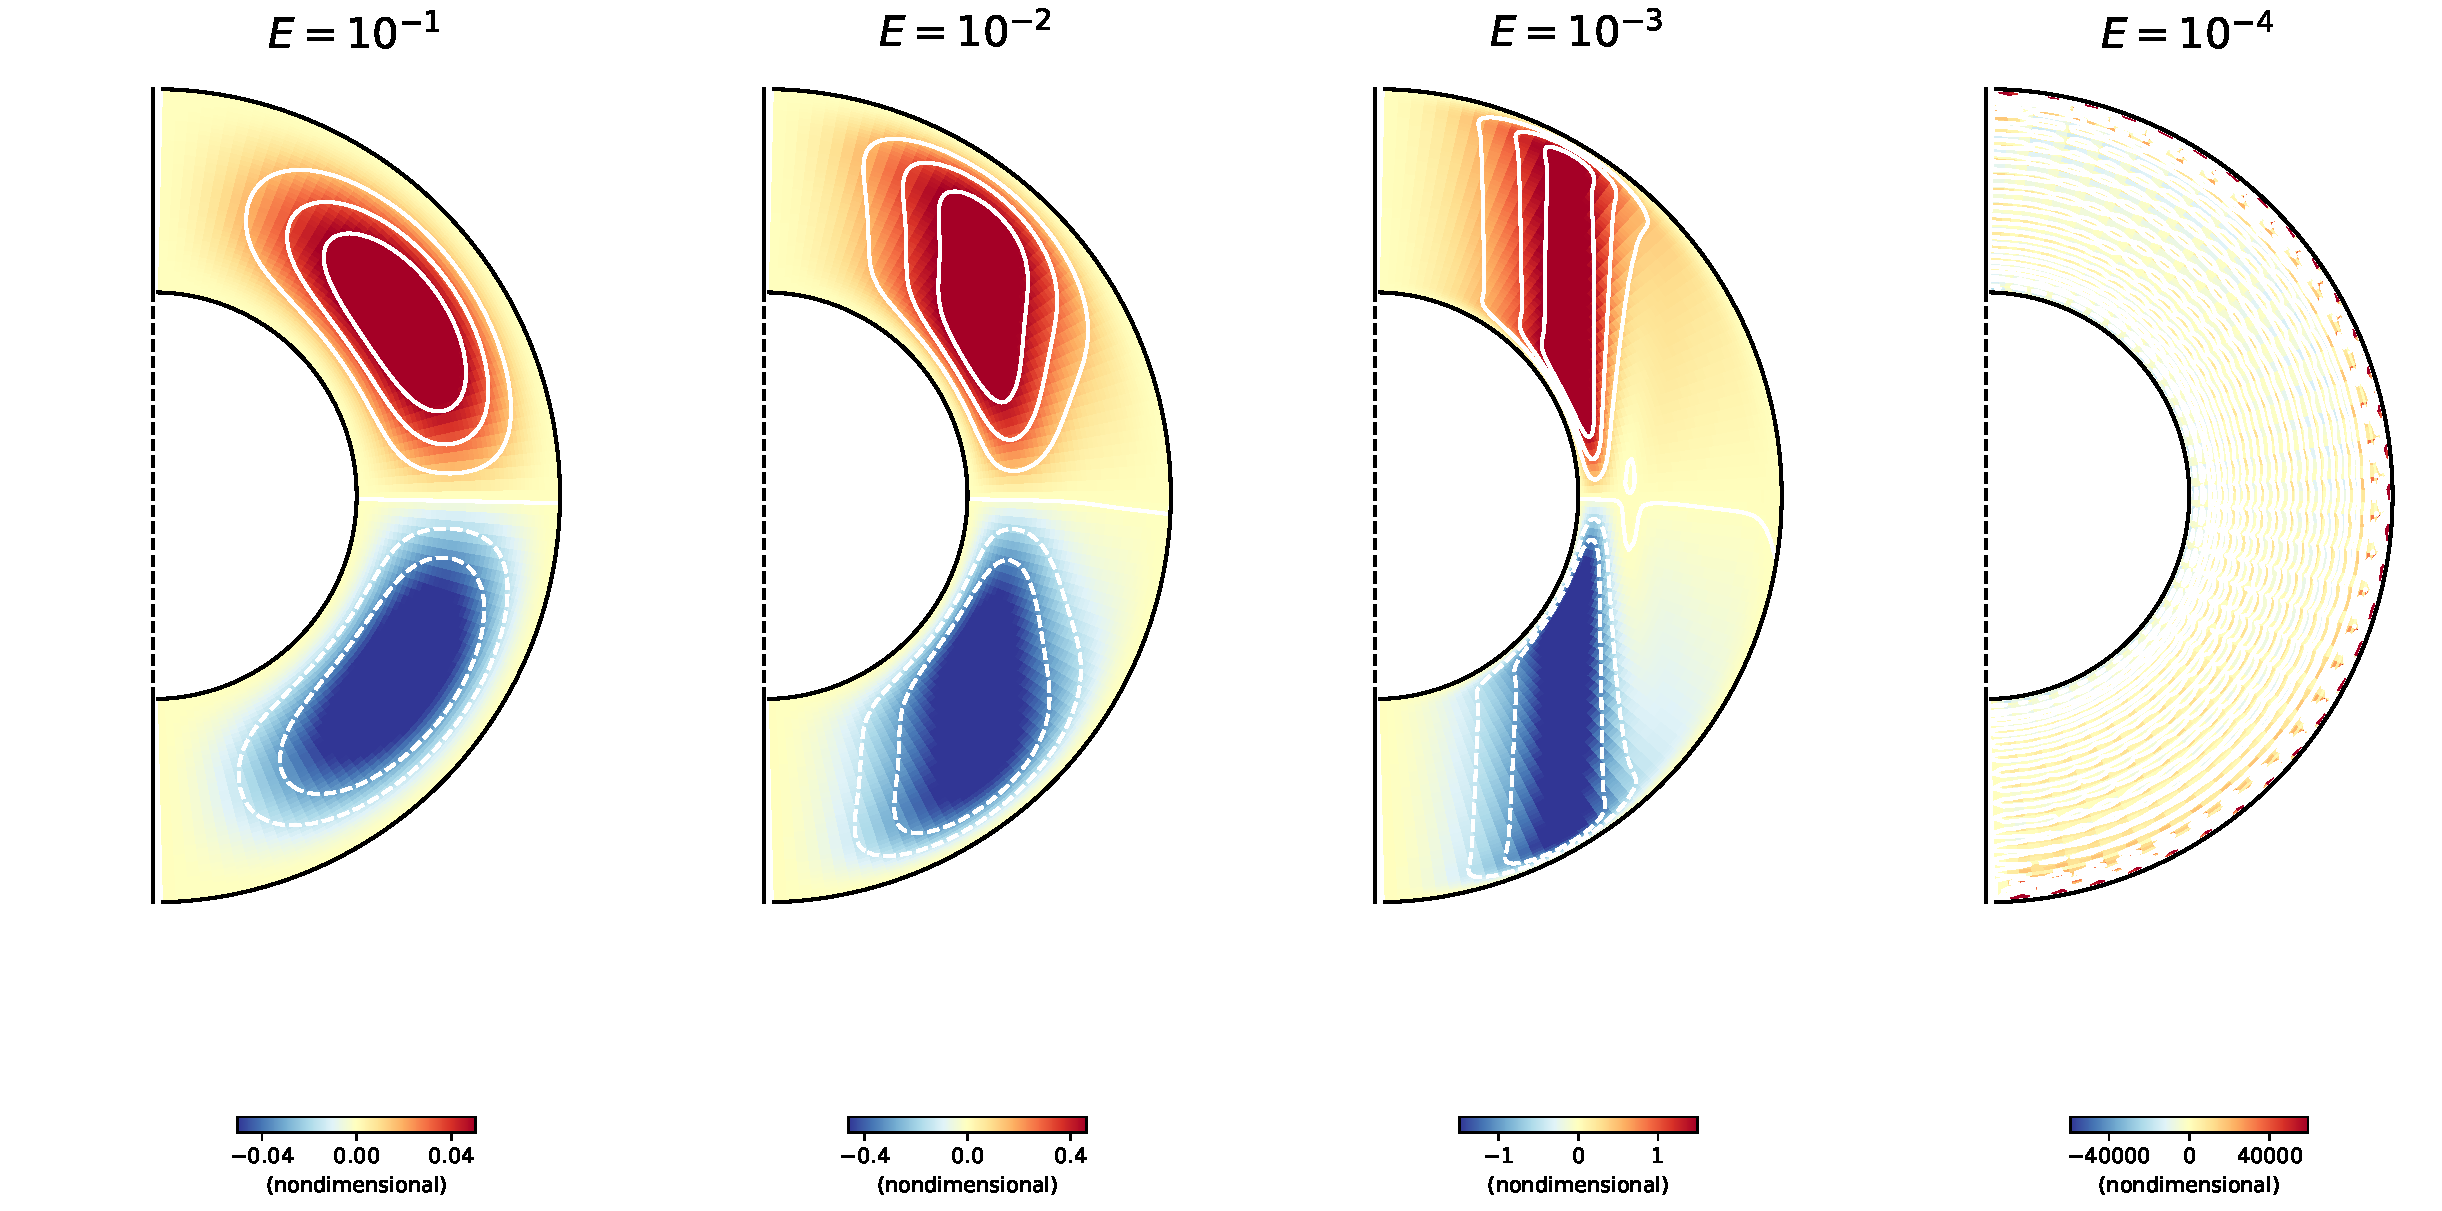
\includegraphics[width=1\textwidth]{figures/AR_0.5/AZ_Avgs_massflux.pdf}
    \caption{Mass flux azimuthal average during equilibrated phase for a range of Ekman numbers.}
    \label{fig:az_avg_massflux_ar_0.5}
\end{figure}
}

\def\condfluxrinarbig{
\begin{figure}[h]
    \centering
    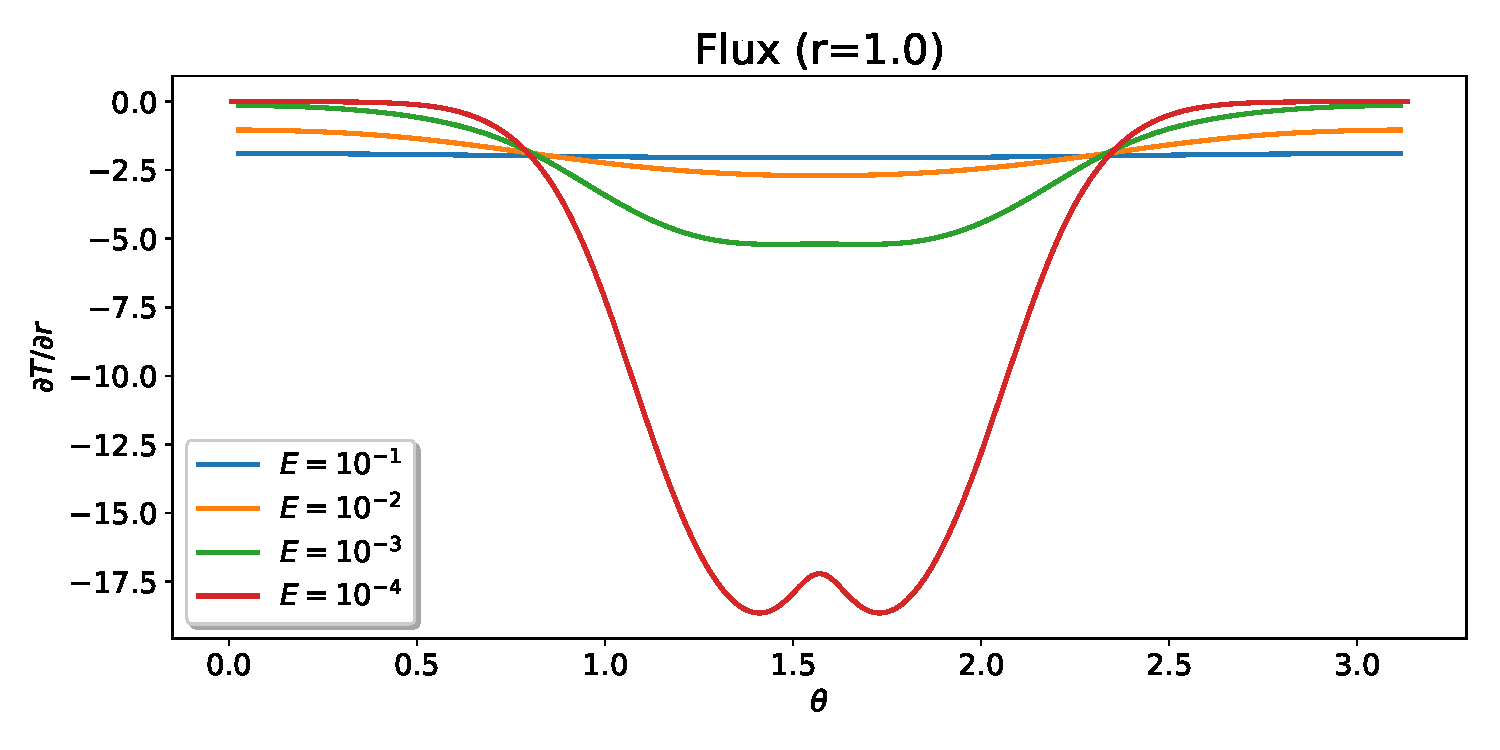
\includegraphics[width=1\textwidth]{figures/AR_0.5/condflux_theta_rin_ar05.pdf}
    \caption{Conductive flux azimuthal average as a function of $\theta$ at the inner radius for a range of Ekman numbers.}
    \label{fig:condflux_rin_big}
\end{figure}
}


\def\condfluxroutarbig{
\begin{figure}[h]
    \centering
    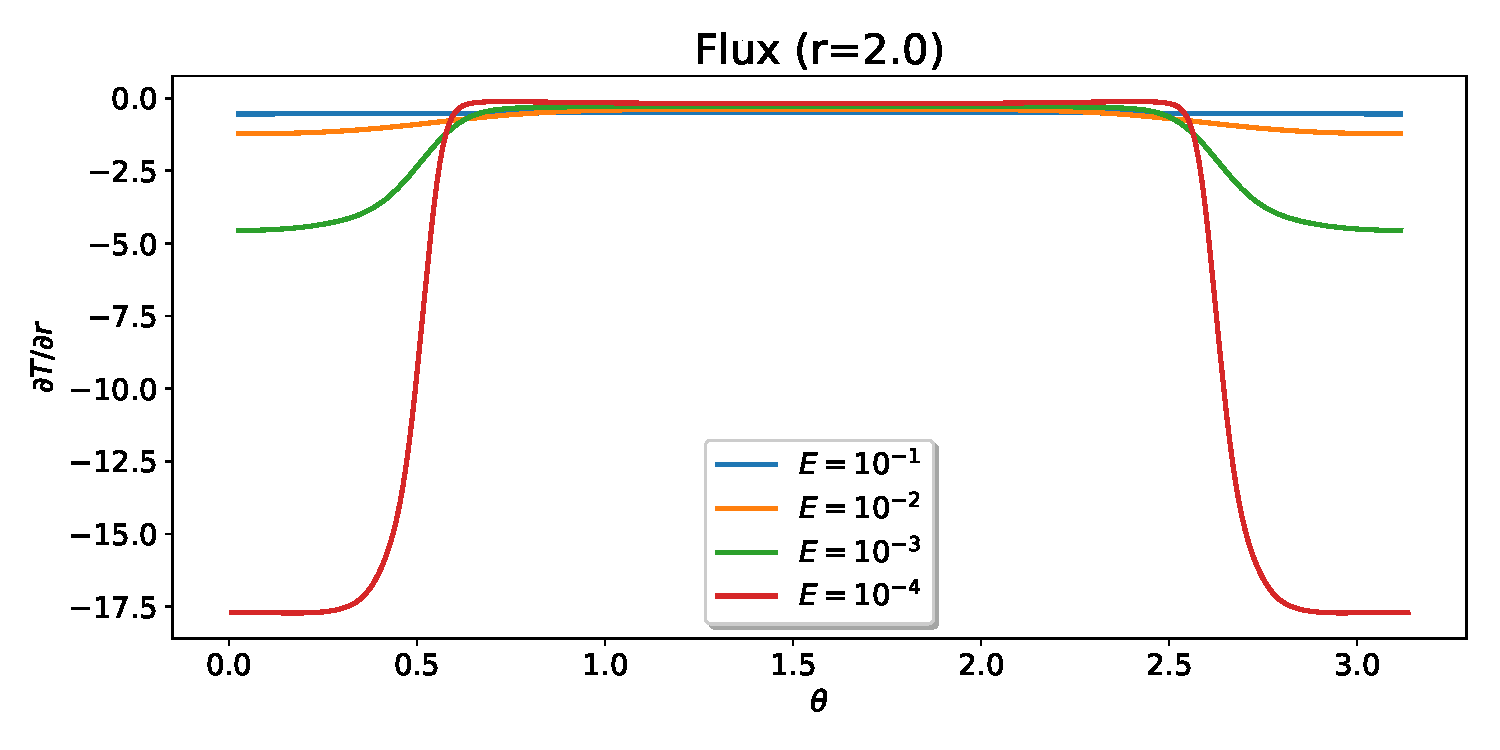
\includegraphics[width=1\textwidth]{figures/AR_0.5/condflux_theta_rout_ar05.pdf}
    \caption{Conductive flux azimuthal average as a function of $\theta$ at the outer radius for a range of Ekman numbers.}
    \label{fig:condflux_rout_big}
\end{figure}
}
